\documentclass[12pt]{article}
\usepackage[margin=0.75in]{geometry}
\usepackage{microtype}
\usepackage{amsmath,amssymb}
\usepackage{array,delarray}
\usepackage[dvips]{graphicx} \usepackage{xspace}
\usepackage{wrapfig}
\usepackage{color}
\usepackage[square,sort&compress,numbers]{natbib}
\usepackage{times}
%\usepackage{caption}
\usepackage{subfig}
%\usepackage{subcaption}
\usepackage{colortbl}
\usepackage[table]{xcolor}
\usepackage{url}
\usepackage{microtype}
\usepackage{nomencl}
\usepackage{algorithm}
\usepackage[noend]{algpseudocode}
\algnewcommand{\Initialize}[1]{%
	\State \textbf{Initialize:}
}


\usepackage{hyperref}
\hypersetup{colorlinks=true,linkcolor=blue,linkcolor=blue,citecolor=blue,urlcolor=blue}

%%
\graphicspath{{./}{./figs/}}

%%\usepackage{citesort}
%\usepackage{sidecap}
%\usepackage{times} % assumes new font selection scheme installed
%\usepackage[small]{caption}




\renewcommand{\thesection}{\Roman{section}}
\renewcommand{\thesubsection}{{\bfseries\Alph{subsection}}}

\DeclareMathOperator*{\argmin}{arg\,min}



\title{Creating synthetic distribution networks}



%%
\begin{document}
	\maketitle
	
	\section{Prior Works}
Previous works by Overbye et al.~\cite{overbye_101,overbye_102} propose methods to generate synthetic transmission network which bear topological and geographical resemblance with a real power system. At first, a statistical study is performed to estimate the per capita power consumption. This, along with the population information from the US Census data is used to estimate the real/reactive power demand at each ZIP code center which is considered to be locations of load substations. This estimated value is used as the substation load and voltage is assigned based on typical values present in the geographic region. Generator location and capacity data obtained from the US Energy Information Administration (EIA) is used to identify locations of generator substations. Thereafter, a Delaunay Triangulation method is used to connect the generator and load substations while maintaining the statistical aspects of a real power system network at the same time. However, these works lack methods to generate multiple number of such realistic synthetic networks. Furthermore, the models aggregate the distribution system to a load substation with an aggregated load value. In our work, we present a method to generate realistic synthetic distribution networks in as much detail as possible.
	\section{Preliminaries}\label{sec:prelim}
In this work, we try to generate the distribution network for a given region (county/town/city) from different open source publicly available information. These data pertain to following sources.
\begin{itemize}
	\item Transportation network data published by NAVTEQ~\cite{navteq}.
	\item Geographical location of high voltage (HV) and extra-high voltage (EHV) substations from data sets published by U.S. Energy Information Administration (EIA)~\cite{eia_substations}.
	\item Residential electric power demand information developed in the models by~\cite{swapna_2018}.
\end{itemize}
The distribution system is synthesized in a way such that it resembles a typical radial distribution feeder network. The goal of this work is to generate the primary and secondary distribution network to connect the substations to all building locations. We want a mapping between the substations and residential locations. This can be achieved by mapping the substations to nodes of the transportation (road) network and assigning a map between residential buildings and road network links. The road network can be used as a proxy for the primary distribution network. The secondary distribution network can be generated from the second map.

The NAVTEQ transportation network data is available in the form of an edge-list or a list of links. Each link $e$ has an associated integer level $l_e$ from the set $\{1,2,3,4,5\}$ that describes the link type (e.g., a level-1 ($l_e=1$) link could correspond to an Interstate road segment, while a level-5 ($l_e=5$) link could correspond to a residential driveway). All links with level $l_e\leq2$ are removed from the dataset. These links are dropped since	components of the distribution network (e.g., homes) are typically not located along these links. Furthermore, connected components in the road network graph of considerable size (number of nodes greater than 10) are only considered. This is done to remove small connected components along which a radial primary distribution feeder network cannot exist.

The synthetic population data and the substation information is available for the entire United States and stored in a database together with the NAVTEQ data. The synthetic distribution network is generated for a particular county. For this purpose, the required data set is selected from the master database based on the zip code information. The available data set is therefore listed as below.
\begin{enumerate}
	\item[(i)] The road network represented in the form of a graph $\mathsf{R}=(\mathsf{V},\mathsf{L})$, where $\mathsf{V}$ and $\mathsf{L}$ are respectively the sets of nodes and links of the network. Each node in the graph has an associated spatial embedding in form of longitude and latitude. 
	\item[(ii)] The set of substations $\mathsf{S}=\{s_1,s_2,\cdots,s_M\}$, where the county consists of $M$ substations and their respective geographical location data.
	\item[(iii)] The set of residential building locations $\mathsf{H}=\{h_1,h_2,\cdots,h_N\}$, where the county consists of $N$ home locations. Each building is associated with longitude-latitude information.
\end{enumerate}


	\section{Algorithm}
\subsection{Constructing the mapping}\label{subsec:map}
\begin{figure}
	\centering
	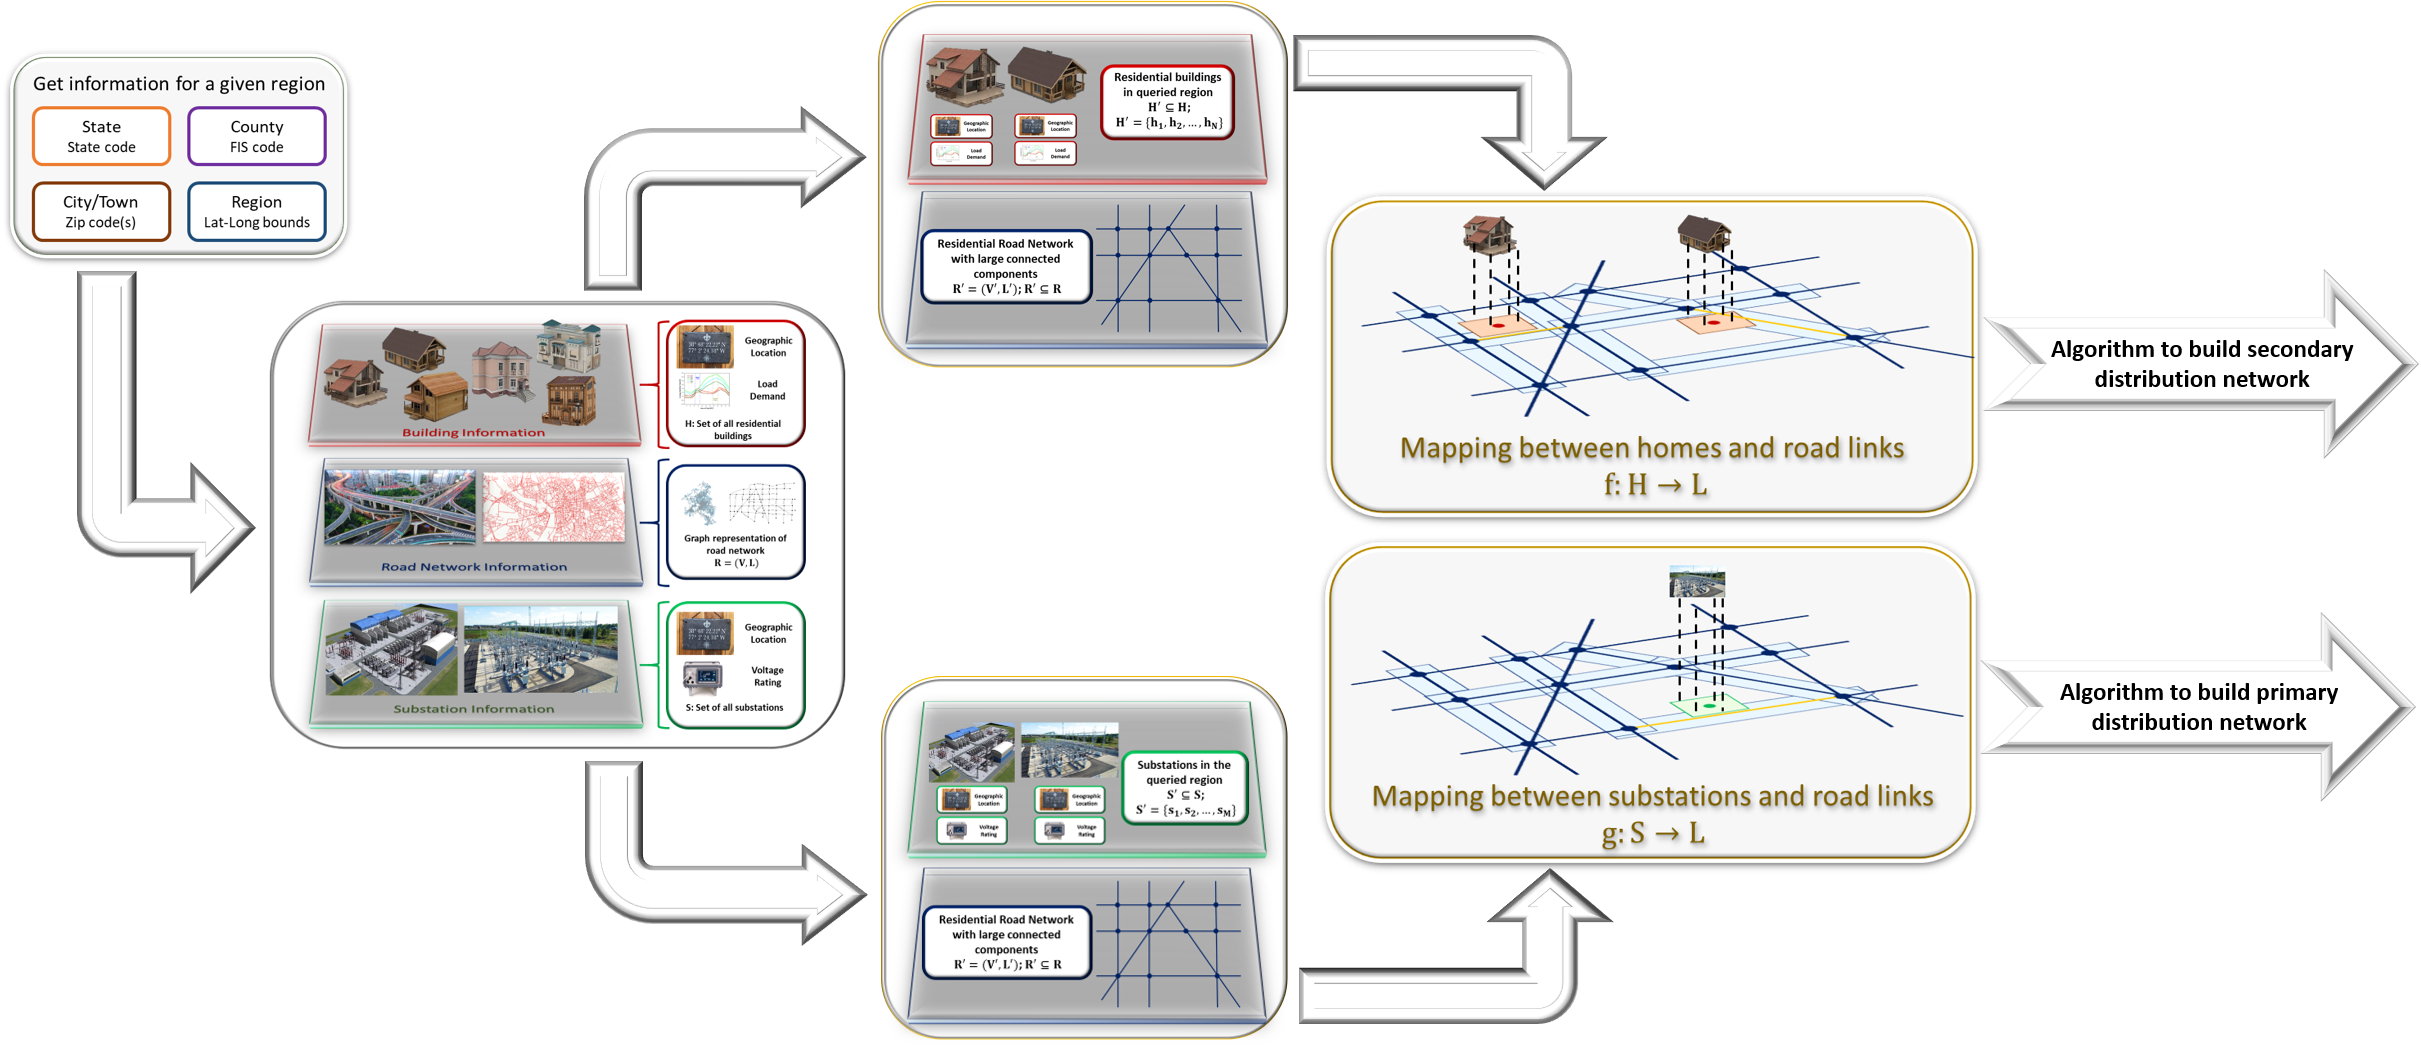
\includegraphics[scale=0.42]{pipeline_1}
	\caption{Flowchart showing the generation of maps between three data sets.}
\end{figure}
\begin{algorithm}[H]
	\caption{Find the nearest link in $\mathsf{L}$ to a given point $\mathbf{p}$.}
	\label{alg:dist}
	\begin{algorithmic}[1]
		\Require Radius for bounding boxes $r$, a mapping $\mathsf{dist}:\mathbb{R}^2\times\mathsf{L}\rightarrow\mathbb{R}^{+}$ such that $\mathsf{dist}(\mathbf{p},\mathbf{l})$ is the shortest distance between point $\mathbf{p}\in\mathbb{R}^2$ and link segment $\mathbf{l}=\mathbf{u}-\mathbf{v}$ for $\mathbf{l}\in\mathsf{L}$ and $\mathbf{u},\mathbf{v}\in\mathbb{R}^2$.
		\For {each link $\mathbf{l}\in\mathsf{L}$}
		\State evaluate bounding box $\mathbf{B_l}$ such that $\mathbf{B_l}=\big\{\mathbf{x}\big|||\mathbf{x}-\mathbf{x_l}||_2\leq r,\forall \mathbf{x_l}=\theta\mathbf{u}+(1-\theta)\mathbf{v},\theta=[0,1]\big\}$.
		\EndFor
		\State Evaluate bounding box $\mathbf{B_p}$ for point $\mathbf{p}$ such that $\mathbf{B_l}=\big\{\mathbf{x}\big|||\mathbf{x}-\mathbf{p}||_2\leq r\big\}$.
		\State Find the bounding boxes $\mathbf{B_{l_1}},\mathbf{B_{l_2}},\cdots,\mathbf{B_{l_m}}$ which intersect with $\mathbf{B_p}$.
		\State Find the link $\mathbf{l^\star}\in\mathsf{L'}$, where $\mathsf{L'}=\{\mathbf{l_1},\mathbf{l_2},\cdots,\mathbf{l_m}\}\subseteq\mathsf{L}$ such that $\mathbf{l^\star}=\argmin_{\mathbf{l}\in\mathsf{L}}\mathsf{dist}(\mathbf{p},\mathbf{l})$.
	\end{algorithmic}
\end{algorithm}
\begin{algorithm}[H]
	\caption{Generate mapping between building and road network data sets.}
	\label{alg:map1}
	\begin{algorithmic}[1]
		\Require Road network graph $\mathsf{R=(\mathsf{V},\mathsf{L})}$, set of residential buildings $\mathsf{H}$, a mapping $\mathsf{dist}:\mathsf{H}\times\mathsf{V}\rightarrow\mathbb{R}^{+}$ such that $\mathsf{dist}(h,v)$ is the Euclidean distance between building $h\in\mathsf{H}$ and road network node $v\in\mathsf{V}$.
		\Initialize :A mapping from road nodes to set of sets of buildings $p:\mathsf{V}\rightarrow\mathcal{H}$ such that $p(v)=\emptyset,\forall v\in\mathsf{V}$
		\For {each building $h\in\mathsf{H}$}
		\State find mapping $f:\mathsf{H}\rightarrow\mathsf{L}$ using Algorithm~\ref{alg:dist} to generate the nearest link $e\in\mathsf{L}$.
		\EndFor
		\For {each link $e=(u,v)\in\mathsf{L}$}
		\State Initialize four sets: $\mathsf{H_{uA}},\mathsf{H_{vA}},\mathsf{H_{uB}},\mathsf{H_{vB}}=\emptyset$.
		\State find the inverse mapping $f^{-1}:\mathsf{L}\rightarrow\mathsf{H}$ which generates the set of buildings $\mathsf{H_e}$ associated with $e$.
		\State find the set of buildings $\mathsf{H_{eA}},\mathsf{H_{eB}}\subseteq\mathsf{H_e}$ with $\mathsf{H_{eA}}\cup\mathsf{H_{eB}}=\mathsf{H_e}$ which are on opposite sides of $e$.
		\For {each building $h\in\mathsf{H_{eA}}$}
		\If {$\mathsf{dist}(h,u)<\mathsf{dist}(h,v)$}
		\State Add this building to set $\mathsf{H_{uA}}$: $\mathsf{H_{uA}}\leftarrow\mathsf{H_{uA}}\cup\{h\}$
		\Else
		\State Add this building to set $\mathsf{H_{vA}}$: $\mathsf{H_{vA}}\leftarrow\mathsf{H_{vA}}\cup\{h\}$
		\EndIf
		\EndFor
		\For {each building $h\in\mathsf{H_{eB}}$}
		\If {$\mathsf{dist}(h,u)<\mathsf{dist}(h,v)$}
		\State Add this building to set $\mathsf{H_{uB}}$: $\mathsf{H_{uB}}\leftarrow\mathsf{H_{uB}}\cup\{h\}$
		\Else
		\State Add this building to set $\mathsf{H_{vB}}$: $\mathsf{H_{vB}}\leftarrow\mathsf{H_{vB}}\cup\{h\}$
		\EndIf
		\EndFor
		\State Add the sets $\mathsf{H_{uA}},\mathsf{H_{uB}}$ to the mapping $p(u)$: $p(u)\leftarrow p(u)\cup\{\mathsf{H_{uA}},\mathsf{H_{uB}}\}$.
		\State Add the sets $\mathsf{H_{vA}},\mathsf{H_{vB}}$ to the mapping $p(v)$: $p(v)\leftarrow p(v)\cup\{\mathsf{H_{vA}},\mathsf{H_{vB}}\}$.
		\EndFor
	\end{algorithmic}
\end{algorithm}

\begin{algorithm}[H]
	\caption{Generate mapping between substations and road network nodes.}
	\label{alg:map2}
	\begin{algorithmic}[1]
		\Require Road network graph $\mathsf{R=(\mathsf{V},\mathsf{L})}$, set of substations $\mathsf{S}$, a mapping $\mathsf{dist}:\mathsf{S}\times\mathsf{V}\rightarrow\mathbb{R}^{+}$ such that $\mathsf{dist}(s,v)$ is the Euclidean distance between substation $s\in\mathsf{S}$ and road network node $v\in\mathsf{V}$, mapping $p:\mathsf{V}\rightarrow\mathcal{H}$ obtained from Algorithm~\ref{alg:map1}, minimum number of road network nodes mapped to a substation $N_{min}$.
		\For {each road network node $v\in\mathsf{V}$}
		\If {$p(v)=\emptyset$}
		\State Remove node $v$ from set of all road network nodes $\mathsf{V}\leftarrow\mathsf{V}\setminus\{v\}$.
		\Else 
		\State Find a mapping $g:\mathsf{V}\rightarrow\mathsf{S}$ which identifies the nearest substation to the road node $v$ such that $g(v)=\argmin_{s\in\mathsf{S}}\mathsf{dist}(s,v)$.
		\EndIf
		\EndFor
		\For {each substation $s\in\mathsf{S}$}
		\State Find inverse mapping $g^{-1}:\mathsf{S}\rightarrow\mathsf{V}$ which generates the set of road network nodes $\mathsf{V_s}$ associated with $s$.
		\If {$|g^{-1}(s)|<N_{min}$}
		\State Remove the substation from set of all substations, $\mathsf{S}\leftarrow\mathsf{S}\setminus\{s\}$
		\EndIf 
		\EndFor
		\State Recompute mapping $g:\mathsf{V}\rightarrow\mathsf{S}$ which identifies the nearest substation to the road node $v$ such that $g(v)=\argmin_{s\in\mathsf{S}}\mathsf{dist}(s,v)$.
	\end{algorithmic}
\end{algorithm}

\begin{figure}[H]
	\centering
	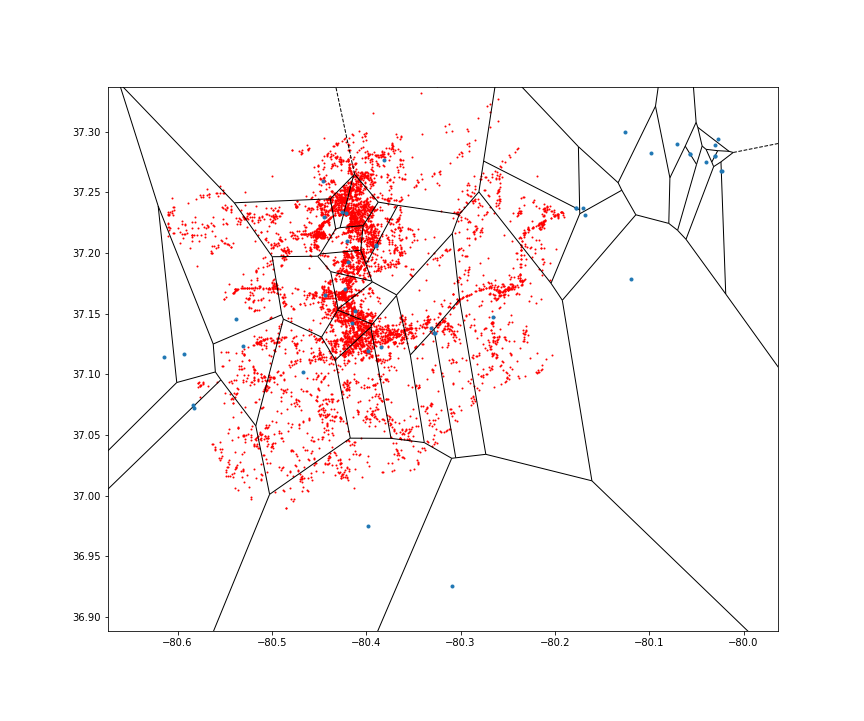
\includegraphics[scale=0.42]{map1}
	\caption{Voronoi regions formed by substations (blue points) and the road nodes (red points) mapped within each region. A number of substations have very road nodes associated with it. Therefore, the Voronoi regions are recomputed after removing the unmapped substations.}
\end{figure}

\begin{figure}[H]
	\centering
	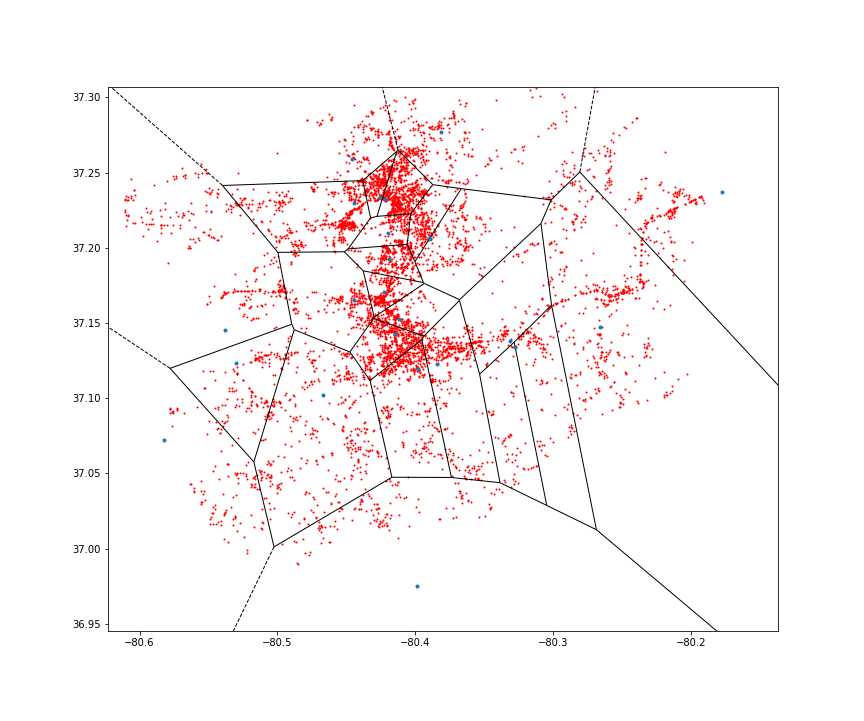
\includegraphics[scale=0.42]{map2}
	\caption{Voronoi regions formed by substations (blue points) and the road nodes (red points) mapped within each region. Almost all the regions are densely distributed by road network nodes. The boundary regions seem to be empty. However, they would be filled by road nodes from the neighboring counties.}
\end{figure}

	
	\bibliographystyle{unsrt}
	\bibliography{references}
	
\end{document}